\subsubsection{Organic Synthesis - New Chiral Amine Building Blocks for Drug Synthesis }
\index{Nugent, Thomas C.}

\paragraph{Research Team}
Dr. Thomas C. Nugent (Professor), Abhijit Ghosh (PhD Student), Vijay Wakchaure (PhD
Student), Mohamed El-Shazly (PhD Student), Christine Holzapfel (Lab Assistant) \\

The Nugent group is interested in the synthesis of organic molecules of consequence, that
is, those having immediate societal impact (pharmaceutical and natural product drugs) and
those containing challenging architectural features.  These molecules require many
chemical operations to synthesize (build) them and sometimes require years of research to
do so.  More often than not, a specific sequence of chemical operations (multistep organic
synthesis) may only be accomplished when new synthetic methods (single organic
transformations) are developed.  In particular synthetic methods based on enantioselective
catalysis, employing transition metals (organometallic catalysts) or organic catalysts,
are at the forefront of our modern know how in synthetic organic chemistry.  Development
of these reactions is important because they enable the transformation of inexpensive
prochiral (i.e. without handedness) organic starting materials into high value chiral
(i.e. with handedness) synthons.  These chiral synthons (building blocks) allow the
efficient synthesis of pharmaceutical and natural product drugs to occur.

\paragraph{Highlights}

In 2006 we completed our initial research findings regarding the use of Ti(OiPr)$_4$ for
the efficient synthesis of aliphatic and aromatic $\alpha-,\alpha$-substituted chiral
primary amines. These high value chiral building blocks are important for natural product
and pharmaceutical drug synthesis.

In this regard, two methods have been fully developed and published on: asymmetric
reductive amination of prochiral ketones and asymmetric sequential amination-alkylation of
aldehydes. Both methods incidentally use the chiral auxiliary (R)- or
(S)-$\alpha$-methylbenzylamine (Scheme) to induce the new stereocenter and both require
two reaction steps to arrive at the primary amine from the carbonyl starting material. The
methods are useful because they obviate the need for isolating imine
intermediates. Additionally, these new methods represent improved methodology over
existing methods because they are stepwise shorter and higher yielding for $\alpha$-chiral
amine synthesis.

Depending on the subclass of $\alpha$-chiral amine desired different ketones,
e.g. alkyl-alkyl (acyclic or cyclic) or aryl-alkyl (acyclic or cyclic), or
carbanion-aldehyde, e.g. alkyl or aryl aldehydes, starting materials will be required. For
example the reductive amination methods excel at producing $\alpha$-chiral primary amine
products in high ee when sterically dissimilar $\alpha$-,$\alpha$-substituents are
present. Thus ketone starting materials of the general structure $R_{S}C(O)CH_3$,
$R_{M}C(O)CH_3$, $R_{L}C(O)CH_3$, $RLC(O)R_S$, are excellent substrates. On the other
hand, the carbanion-aldehyde (sequential amination-alkylation of aldehydes) method excels,
in terms of yield and de, when two similarly sized substituents are at the stereocenter
adjacent to a nitrogen atom in the amine product. Thus for the latter, combining a
carbanion source $(R_S or R_M)$ with an aldehyde of general structure $R_{S}C(O)H$ or
$R_{M}C(O)H$ or $R_{L}C(O)H$, will allow high diastereoselectivity in products% \textbf{2}
. At the present stage of development, it can be stated that the two strategies (reductive
amination vs \emph{in situ} imine-carbanion addition) complement one another.
\\
Regarding the heterogeneous hydrogenation catalyst (Raney Ni, Pt-C, Pd-C, Ru-C, or Rh-C),
specific classes of ketone substrates emerged as requiring specific catalysts for optimal
stereoselectivityduring reductive amination. The classifications are as follow:
\begin{enumerate}
\item Raney Ni substrates are acyclic alkyl-alkyl or acyclic aryl-alkyl ketones that lack
  an $\alpha$-tertiary carbon, e.g. t-butyl moiety, directly attached to the carbonyl
  carbon;
\item Pt-C substrates are acyclic or cyclic alkyl-alkyl ketones that contain a high degree
  of $\alpha$-carbonyl steric congestion, e.g. pinacolone or 2,2-dimethylcyclopentanone;
  and
\item Pd-C substrates are cyclic aryl-alkyl ketones (benzocyclic) ketones,
  e.g. $\alpha$-tetralone and benzosuberone. General experimental protocols have been
  established for these different classes of ketones, and readily allow semi-optimized
  conditions to be established for yet untested by similarly functionalized prochiral
  ketones.
\end{enumerate}

During 2006 we also started cursory investigations regarding the viability of using other
Lewis acids than $Ti(OiPr)_4$ for reductive amination. This investigation is motivated by
desire to find reaction rate enhancement effects and/or increased stereoselectivity for
amines \textbf{2}. Our early investigations have shown that $B(OiPr)_3$ $Al(OiPr)_3$, and
$Zr(OiPr)_4$ are useful alternatives, but generally lengthen the reaction time for the
reductive amination protocols.

\begin{figure}[ht]
  \begin{center}
    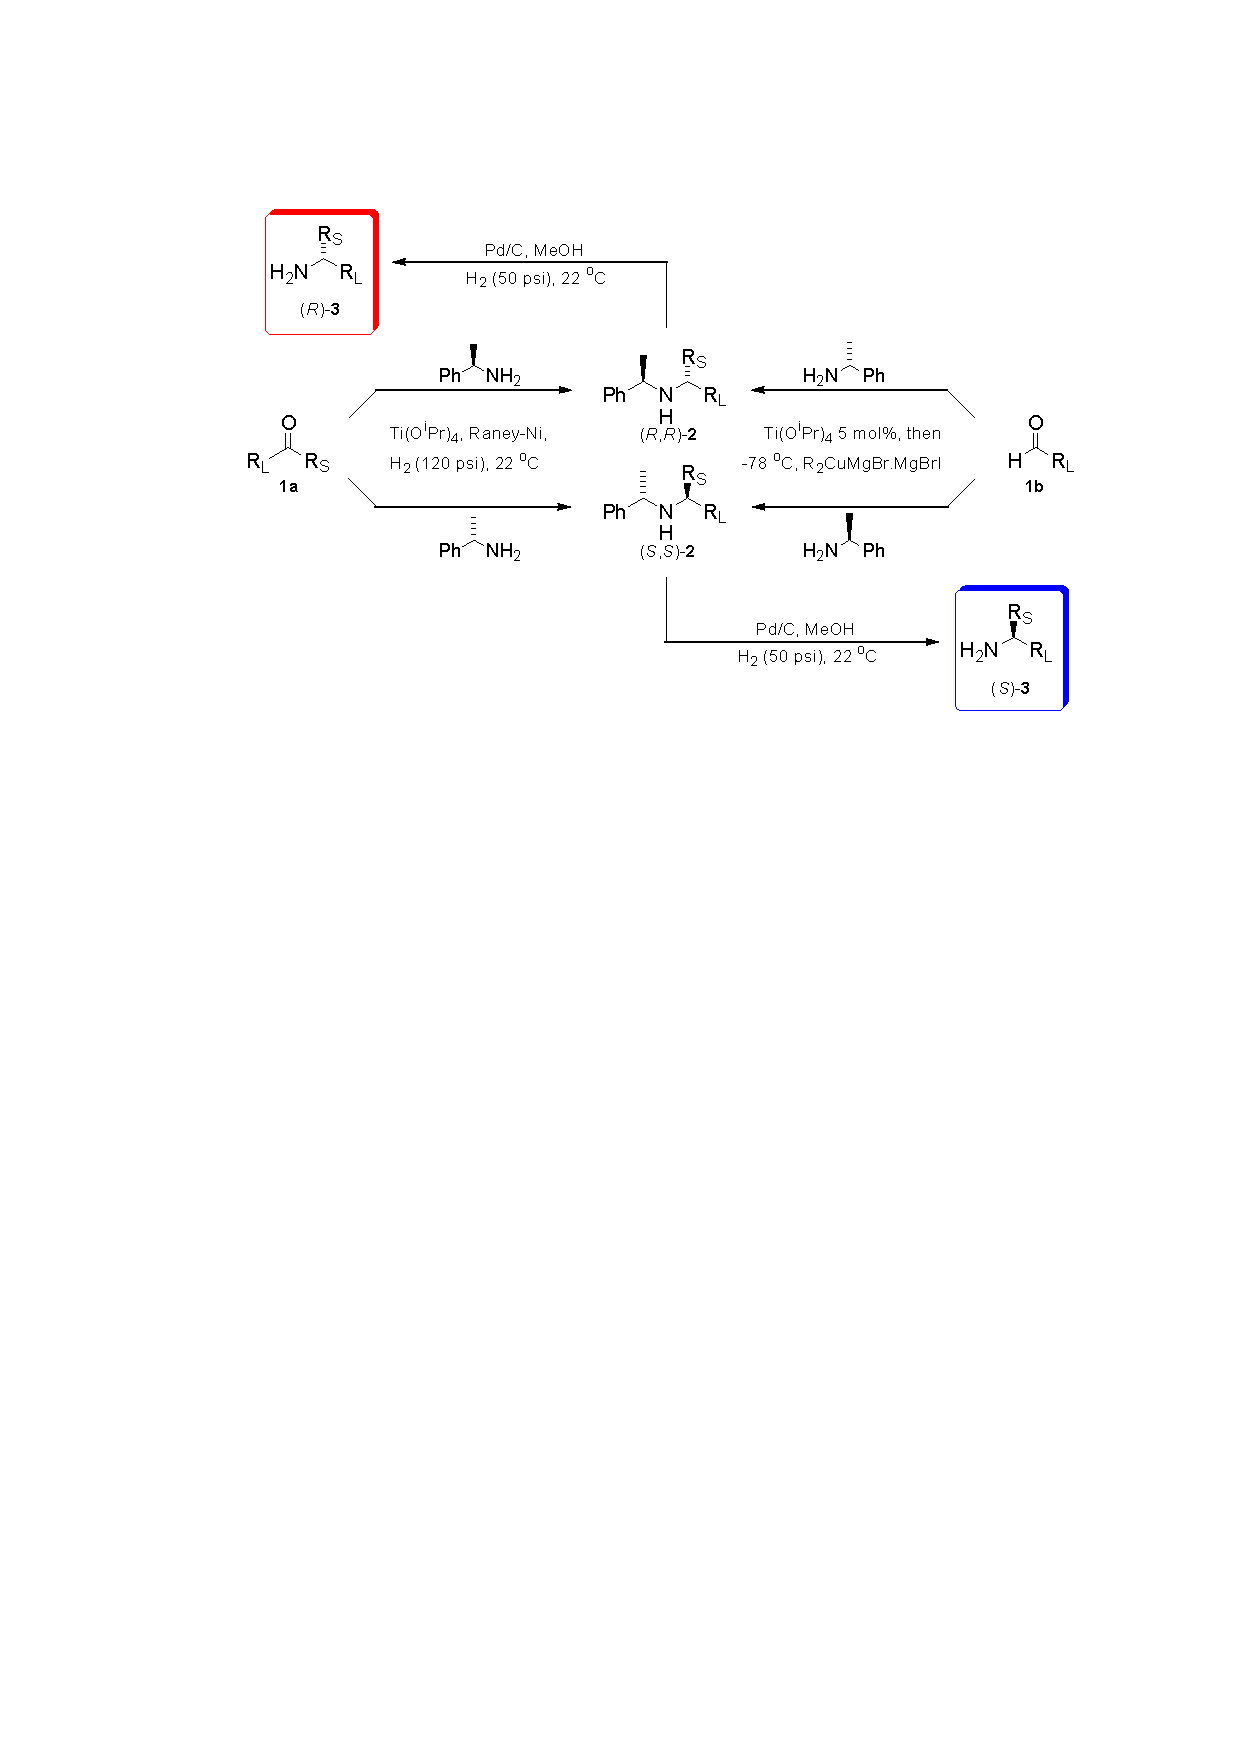
\includegraphics[width=\hsize]{/Nugent/Nugent_2006_Figure.pdf}
    \mycaption{Reductive Amination and Carbanion Methods for Chiral Amine
      Synthesis}\label{fig:profNugent}
  \end{center}
\end{figure}

\paragraph{Patents}
\begin{enumerate}
\item Synthesis of Amine Stereoisomers; Nugent, T. C.; Wakchaure, V. N.; Ghosh, A. K.;
  Mohanty, R. R.(International University Bremen, GmbH), publication number: WO2006030017,
  23 March 2006. 
\end{enumerate}

\nocite{Nugent1}
\nocite{Nugent2}
\nocite{Nugent3}
